\documentclass[aspectratio=169]{beamer}
\usepackage[T1]{fontenc}
\usepackage[default]{sourcesanspro}
\usepackage{newtxsf}
\usepackage{hyperref}
\usepackage{latexsym,amsmath,xcolor,multicol,booktabs,calligra}
\usepackage{graphicx,pstricks,listings,stackengine}
\graphicspath{{./figures/}}
\usepackage{lipsum}
\usepackage{wrapfig}
\usepackage{url}
\usepackage{subcaption}
\usepackage{listings}
\usepackage{minted}
\setminted{fontsize=\footnotesize}
\usepackage{fontawesome5}

\usepackage{etoolbox}

\author{Yan Lin}
\title{AI Systems \& Infrastructure}
\subtitle{Module B.1: AI Hardware Infrastructure}
\institute{%
    \href{https://www.yanlincs.com}{www.yanlincs.com}
}
\date{September 1st, 2026}
\usepackage{AAU}
\AtBeginSubsection{}
\setbeamertemplate{navigation symbols}{}

\def\cmd#1{\texttt{\color{red}\footnotesize $\backslash$#1}}
\def\env#1{\texttt{\color{blue}\footnotesize #1}}
\definecolor{aauyellow}{RGB}{167, 131, 55}
\definecolor{aaublue}{RGB}{32, 26, 78}
\definecolor{aaured}{RGB}{152, 43, 28}
\definecolor{textgrey}{RGB}{60, 60, 60}

\setbeamercolor{normal text}{fg=textgrey}
\usebeamercolor[fg]{normal text}

\def\emphasis#1{{\color{aaured}\textbf{#1}}}
\renewcommand{\thefootnote}{}


\lstset{%
    basicstyle=\ttfamily\small,
    keywordstyle=\bfseries\color{deepblue},
    emphstyle=\ttfamily\color{deepred},
    stringstyle=\color{deepgreen},
    numbers=left,
    numberstyle=\small\color{halfgray},
    rulesepcolor=\color{red!20!green!20!blue!20},
    frame=shadowbox,
}

\begin{document}

\begin{frame}[plain,noframenumbering]
    \titlepage
    \vspace*{-0.6cm}
    \begin{figure}[htpb]
        \begin{center}
            
\includegraphics[keepaspectratio, scale=0.5]{aau-logo-left-uk}
        \end{center}
    \end{figure}
\end{frame}

\begin{frame}
\tableofcontents[sectionstyle=show,
subsectionstyle=show/shaded/hide,
subsubsectionstyle=show/shaded/hide]
\end{frame}


\section{Why Think About Hardware}

% TODO: Add a "Recap: where we are" slide, and an introduction to part B

\begin{frame}{The marketing claim and the reality}
    Vendors love to slap AI onto every new device.
    Marketing pages keep talking about AI computers and AI-ready laptops as if a new kind of machine has been invented just for the hype.

    \vspace{0.5em}
    The reality is much less dramatic.
    \begin{itemize}
        \item In 1945, John von Neumann sketched a design that would become the basis for almost every general-purpose computer built since
        \item Eighty years later, smartphones, gaming PCs, our laptops, even those new AI computers all follow the same design
        \item The hardware has gotten faster, smaller, and cheaper, but the basic recipe has not changed
    \end{itemize}
\end{frame}

\begin{frame}{Two questions for this module}
\begin{enumerate}
\item How is a general-purpose computer actually put together?
\item Where does that design fall short for AI workloads, and what kinds of specialized chips have been added to fill those gaps?
\end{enumerate}

    \vspace{0.5em}
    We use a restaurant kitchen as a running analogy throughout.
\end{frame}


\section{Von Neumann Architecture}

\begin{frame}{The kitchen}
    Imagine a busy kitchen with everything that goes on inside it.

    \begin{itemize}
        \item Orders and recipes coming in
        \item Ingredients ready to be cooked
        \item Chefs preparing dishes
        \item A pantry that stores both ingredients and recipe books
        \item Waiters carrying orders in and food out
        \item Corridors connecting every part of the kitchen
    \end{itemize}

    \vspace{0.5em}
    Each role maps to a component in the architecture.
\end{frame}

\begin{frame}[fragile]{Instructions and data}
    Two kinds of information flow through the kitchen and the computer.

    \begin{block}{Instructions: the recipe}
        A step-by-step description of how to handle ingredients and tools.

\begin{minipage}[t]{0.48\textwidth}
\begin{minted}{text}
1. Cut the onion into pieces.
2. Heat the pan to medium heat.
3. Add 2 tablespoons of oil.
4. Sauté the onions until golden.
\end{minted}
\end{minipage}
\hfill
\begin{minipage}[t]{0.48\textwidth}
\begin{minted}{text}
1. LOAD dkk_price
2. MULTIPLY dkk_price by conversion_factor
3. STORE the result in usd_price
4. DISPLAY usd_price
\end{minted}
\end{minipage}

    \end{block}

    \begin{block}{Data: the ingredients}
        The information the instructions operate on.

\begin{minipage}[t]{0.48\textwidth}
\begin{minted}{text}
- 2 large onions
- Olive oil
\end{minted}
\end{minipage}
\hfill
\begin{minipage}[t]{0.48\textwidth}
\begin{minted}{text}
- dkk_price: 599
- conversion_factor: 0.1570
- usd_price: to be calculated
\end{minted}
\end{minipage}

    \end{block}

\end{frame}

\begin{frame}{The architecture, at a glance}
    \begin{figure}[htpb]
        \begin{center}
            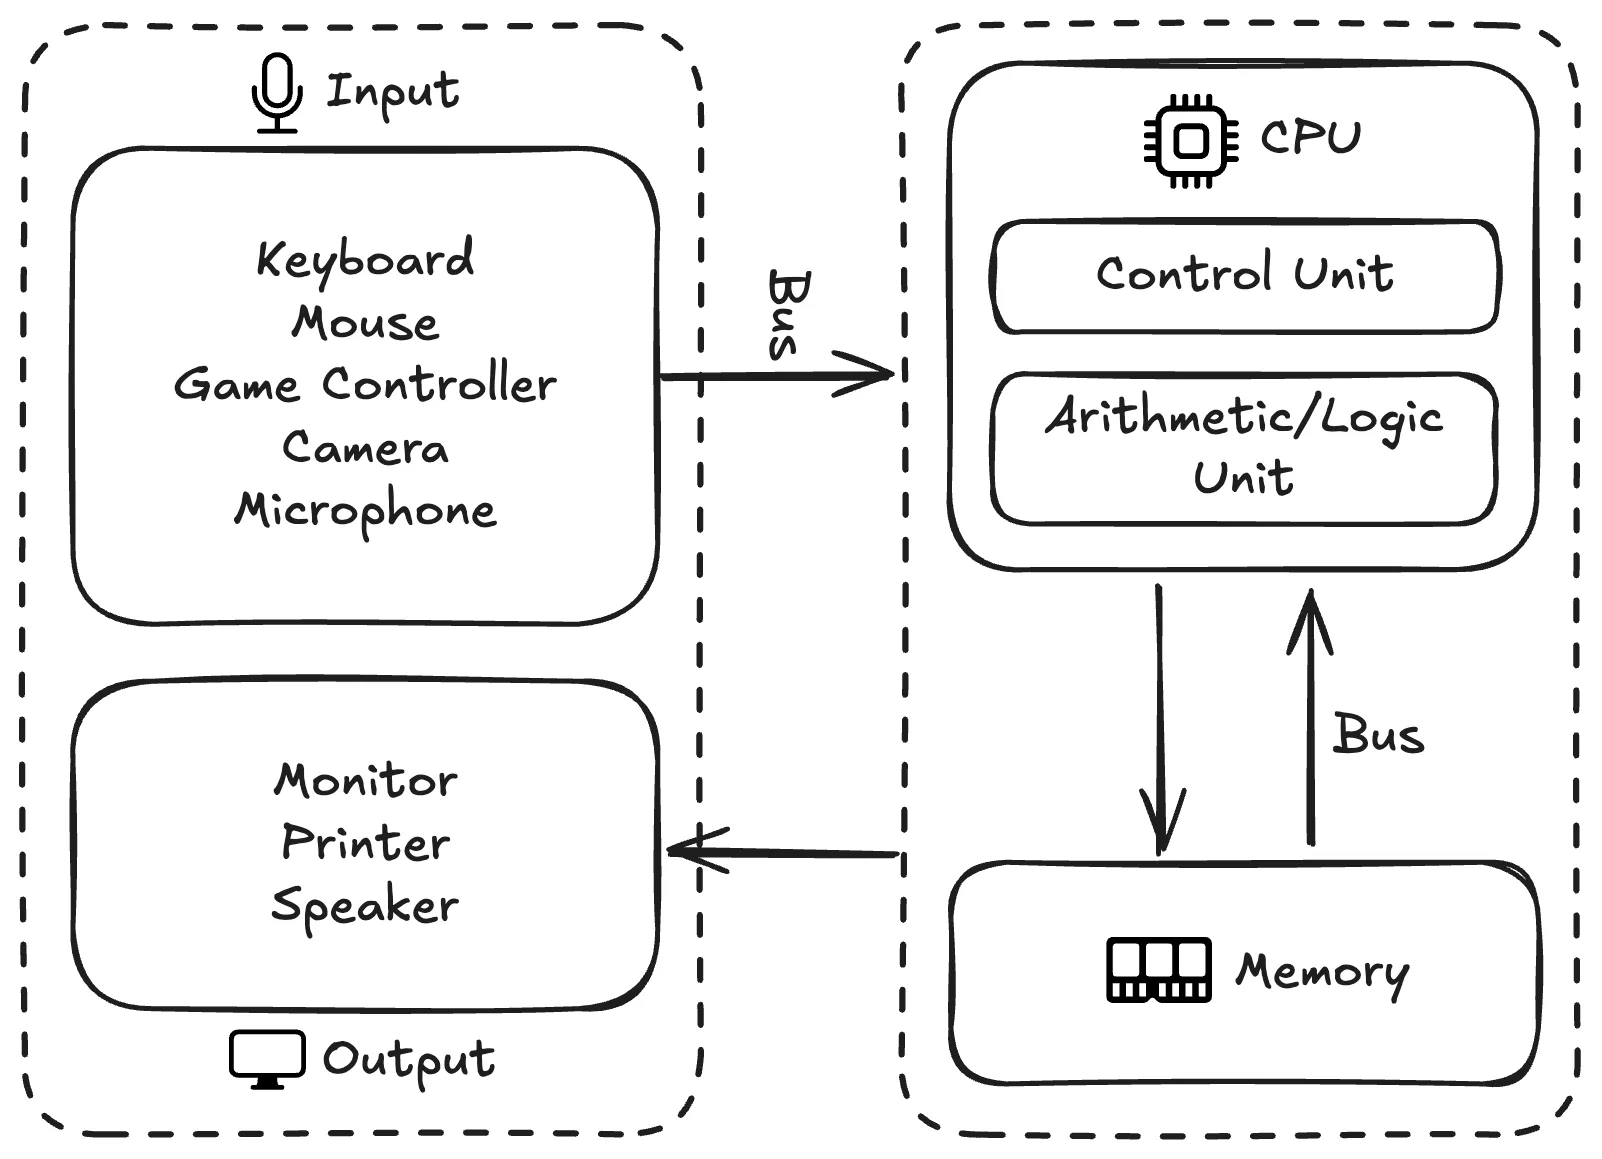
\includegraphics[width=0.6\textwidth]{von-neumann}
        \end{center}
    \end{figure}
\end{frame}

\begin{frame}{CPU: the chefs}
    The \textbf{Central Processing Unit} executes instructions on data.
    Like the chefs who follow recipes to turn ingredients into dishes.

    \begin{block}{Control unit, the executive chef}
        Reads orders and recipes, figures out what needs to happen next, tells everyone else what to do.
        Fetches the next instruction, decodes it, signals the rest of the CPU to carry it out.
    \end{block}

    \begin{block}{Arithmetic logic unit, the cooks}
        Performs the elementary operations that make up every program: arithmetic, logic, comparisons, bit manipulation.
        A modern CPU usually contains more than one ALU per core.
    \end{block}
\end{frame}

\begin{frame}{Memory: the pantry}
    Holds both instructions and data.
    Like a pantry that stores both recipe books and ingredients on the same shelves.

    \begin{itemize}
        \item Every cell has a numerical address, so the CPU can ask for any specific value directly
        \item \emph{Random-access}: any address can be reached in roughly the same time
        \item \emph{Volatile}: turning the power off wipes the contents
    \end{itemize}

    \vspace{0.5em}
    Volatility is why our unsaved work disappears when the computer crashes.
\end{frame}

\begin{frame}{I/O: the waiters}
    The \textbf{input/output system} is how data and programs come into the computer from the outside world, and how results go back out.
    Like the waiters who carry orders into the kitchen and dishes out to the customers.

    \begin{itemize}
        \item Input: keyboards, mice, microphones, cameras
        \item Output: monitors, speakers, printers
        \item Both: network cards, storage drives
    \end{itemize}

Each \textbf{I/O device} is connected through a small piece of hardware called an \textbf{I/O controller} that takes care of the device-specific details, so the rest of the computer can treat all of them in a relatively uniform way.
\end{frame}

\begin{frame}{Bus: the corridors}
    The set of wires that move instructions and data between every other component.
    Like the corridors and counters that let staff and trolleys carry orders, ingredients, and dishes around the kitchen.

    \begin{figure}[htpb]
        \begin{center}
            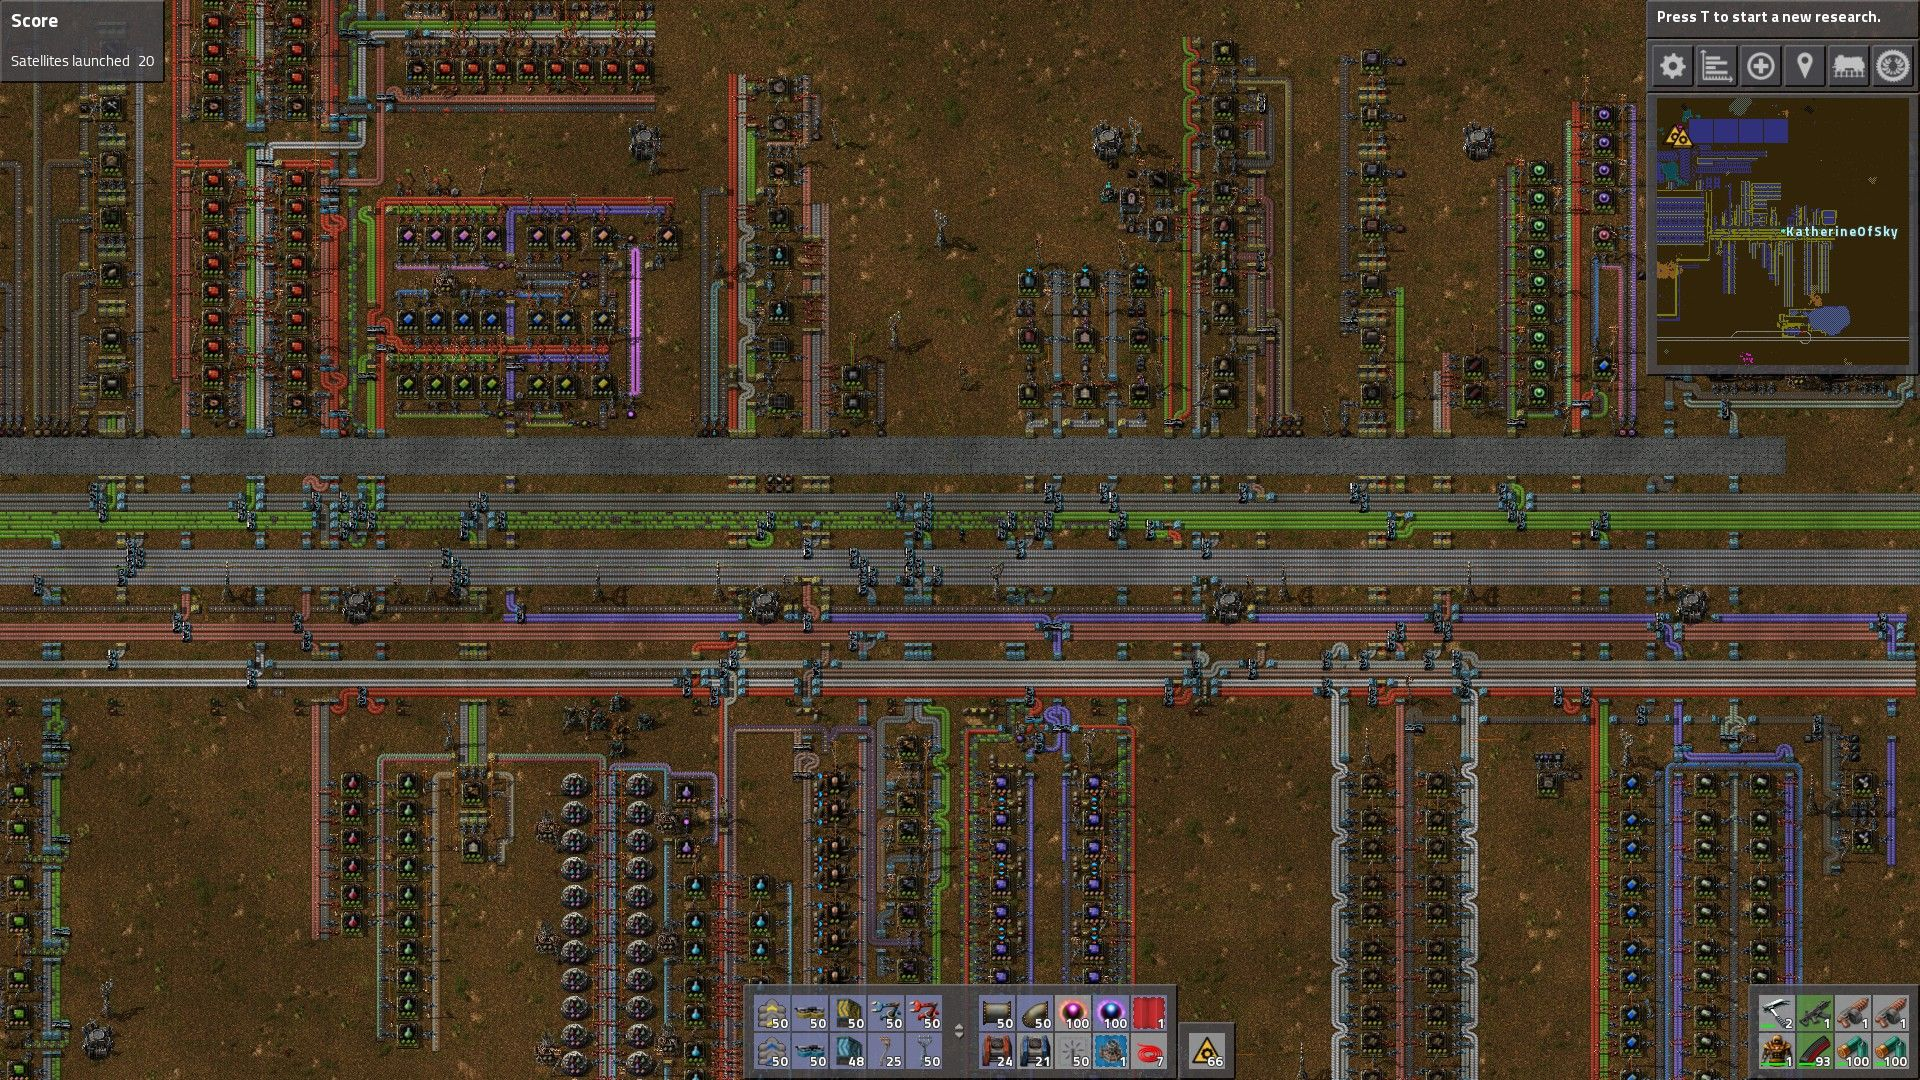
\includegraphics[width=0.5\textwidth]{factorio-bus}
        \end{center}
    \end{figure}

    Three logical parts: address bus (which location), data bus (the actual contents), control bus (timing and coordination).
\end{frame}

\begin{frame}{Tracing through one program}
    The DKK to USD converter from earlier.

    \begin{enumerate}
        \item I/O loads the program and the input value (\texttt{dkk\_price=599}) into memory
        \item Control unit fetches \texttt{LOAD dkk\_price}, tells the CPU to bring 599 into itself
        \item Control unit fetches \texttt{MULTIPLY}, ALU computes 599 * 0.1570 = 94.04
        \item Result is stored back into memory and sent to I/O for display
    \end{enumerate}

    \vspace{0.5em}
A modern Von Neumann architecture computer repeats this loop billions of times per second.
\end{frame}

\begin{frame}{Example: Raspberry Pi 5}
A credit card-size Von Neumann architecture computer.

    \begin{figure}[htpb]
        \begin{center}
            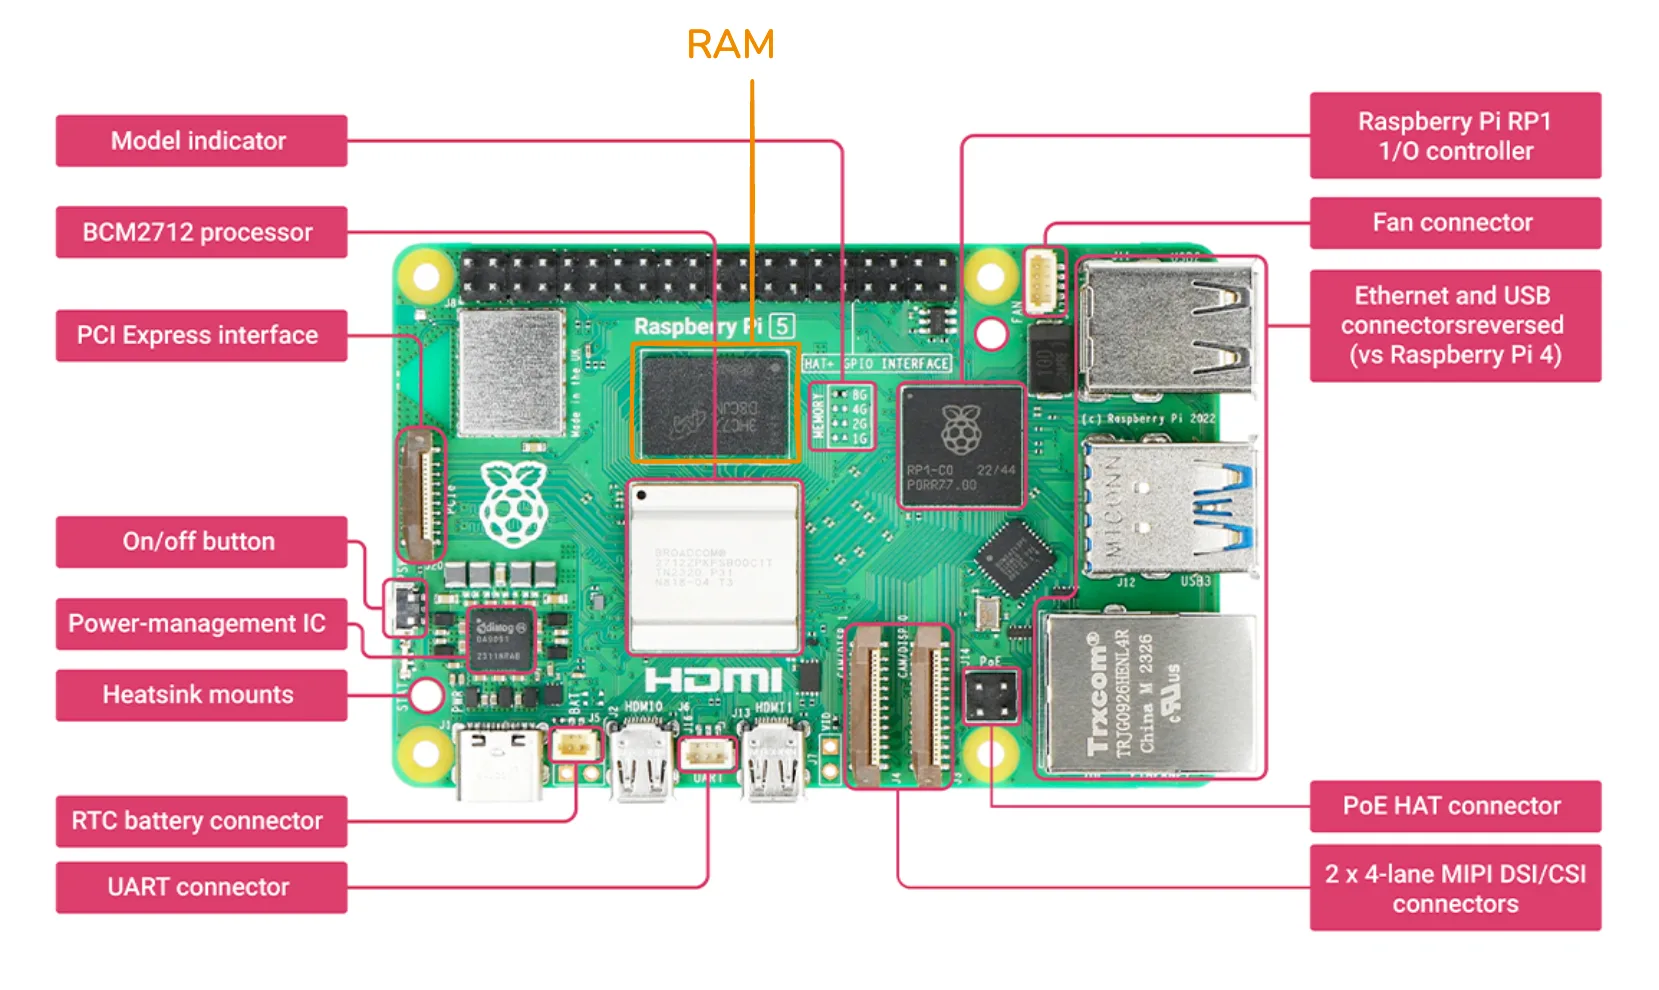
\includegraphics[width=0.6\textwidth]{raspberry-pi}
        \end{center}
    \end{figure}

    CPU in the middle, RAM next to it, I/O around the edges, copper traces between them serve as the bus.
\end{frame}


\section{Where Generic Hardware Falls Short}

\begin{frame}{Two limitations for AI workloads}
    The architecture above describes a \emph{general-purpose} computer.
    It can run anything you throw at it: web browsers, video games, spreadsheets, compilers, and AI models, but not always in the most efficient way.

    \begin{block}{1. Sequential speed vs parallel demand}
        CPUs are tuned for sequential execution, finishing one instruction quickly before the next.
        AI workloads usually heavily demand parallel compute.
    \end{block}

    \begin{block}{2. Memory bandwidth bottleneck}
        Even when the CPU is fast enough to compute, it often spends most of its time waiting for data to arrive from memory.
    \end{block}
\end{frame}

\begin{frame}{Sequential CPU vs parallel work}
Most of the math inside a neural network is \textbf{matrix multiplication}.
    For a single matrix multiplication there can be hundreds of thousands of these tiny calculations, and none of them depend on each other.

    \vspace{0.5em}
A CPU faced with this kind of work is a bit like a \textit{university professor} faced with a giant stack of basic arithmetic worksheets.
    Each problem is well below the professor's pay grade, but solving them one by one still takes forever.

    \vspace{0.5em}
A whole class of \textit{primary school students}, each only able to do basic arithmetic, can power through the same stack much faster.
\end{frame}

\begin{frame}{The memory wall}
There are two opposing aspects of memory performance.

\begin{itemize}
    \item \textbf{Latency}: how long a single piece of data takes to arrive once requested
    \item \textbf{Bandwidth}: how much data can be moved per second
\end{itemize}

A CPU's memory is built around low latency at the cost of bandwidth. Typical DDR5 peaks at around 50 to 100 GB/s.

For modern AI models, we want to load a large chunk of data into the memory as fast as possible, which biases towards memory bandwidth.
\end{frame}


\section{Specialized Hardware for AI}

\begin{frame}{Where the chips come in}
    The two limitations point to the same conclusion.
    AI workloads need hardware that are designed to efficiently handle AI computing workloads.

    \begin{itemize}
        \item Many simple operations in parallel
        \item High-bandwidth memory to feed them
    \end{itemize}

    \vspace{0.5em}
    Several families of chips have been built around this idea, each at a different sweet spot of generality and efficiency.
\end{frame}

\begin{frame}{Graphics Processing Unit (GPU)}
    As the name suggests, GPUs were originally designed for computer graphics, not AI.

    Rendering a 3D scene means computing the color of millions of pixels every frame, each independent of the rest, same workloads as AI models.

    \begin{figure}[htpb]
        \begin{center}
            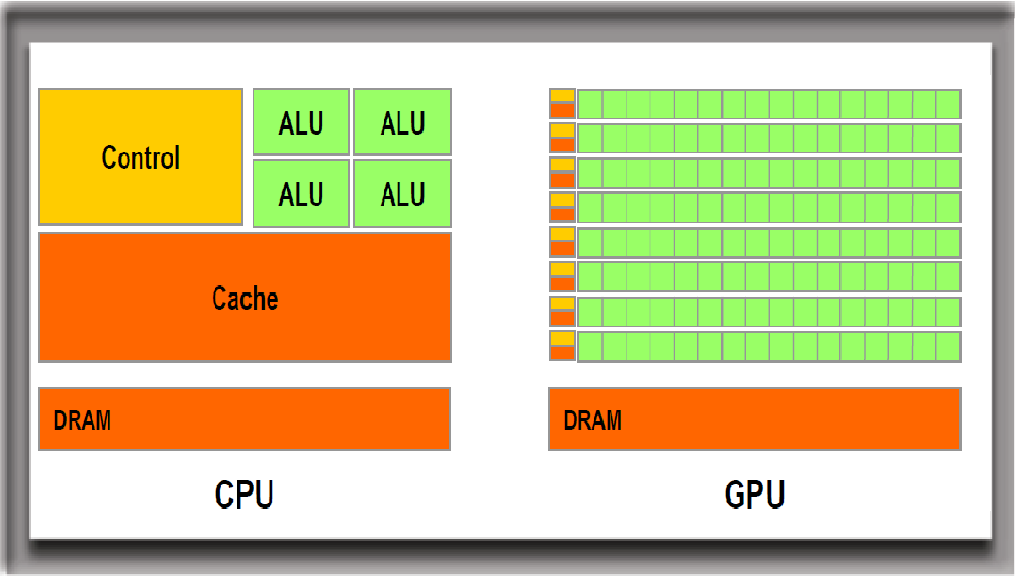
\includegraphics[width=0.5\textwidth]{cpu-gpu}
        \end{center}
\caption*{A GPU usually comes with thousands of small cores, plus memory built for bandwidth (GDDR7 around 1.8 TB/s, HBM above 2 TB/s).}
    \end{figure}
\end{frame}

\begin{frame}{Tensor Processing Unit (TPU)}
    GPUs are still general-purpose enough to handle graphics, scientific simulation, and video encoding.
    That generality can limit how efficient they can be on AI workloads.

\vspace{0.5em}
    Google's \textbf{TPUs} are a type of hardware built specifically for AI model computing.

    \begin{figure}[htpb]
        \begin{center}
            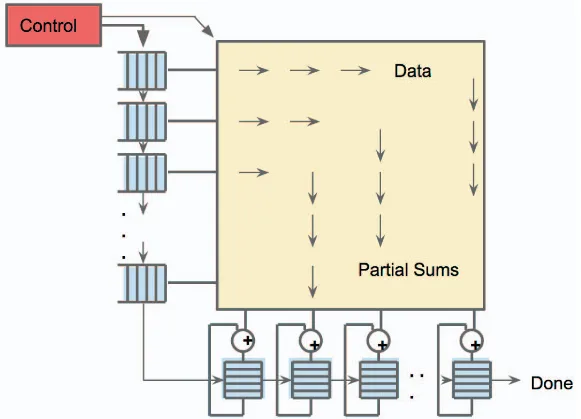
\includegraphics[width=0.35\textwidth]{tpu-architecture}
        \end{center}
    \end{figure}

In reality, GPUs still dominate in specialized hardware for AI computing.
\end{frame}

\begin{frame}{Neural Processing Unit (NPU)}
    GPUs and TPUs both target high end computing.
    NPUs target the low end: consumer devices like phones, tablets, and laptops.

    \begin{itemize}
        \item Built for \emph{inference}, not training
        \item Lower-precision arithmetic, often 8-bit or even 4-bit
        \item Smaller circuits, lower power draw
    \end{itemize}

    \begin{figure}[htpb]
        \begin{center}
            \begin{subfigure}{0.35\textwidth}
                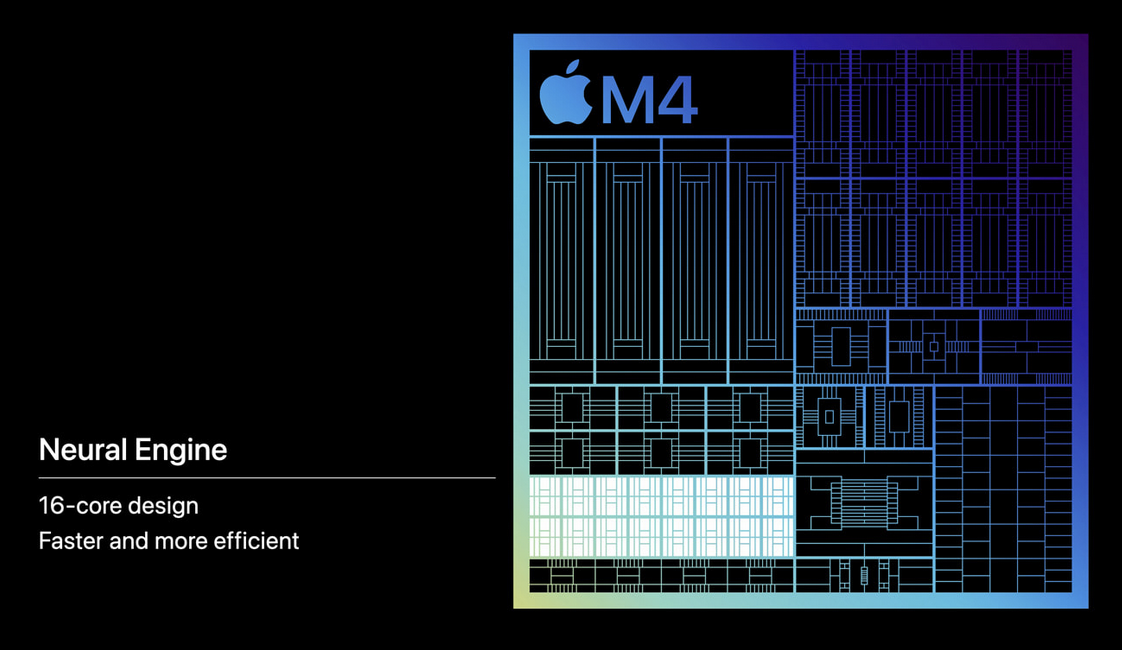
\includegraphics[width=\textwidth]{apple-npu}
                \caption{Apple Neural Engine}
            \end{subfigure}
            \hspace{0.05\textwidth}
            \begin{subfigure}{0.4\textwidth}
                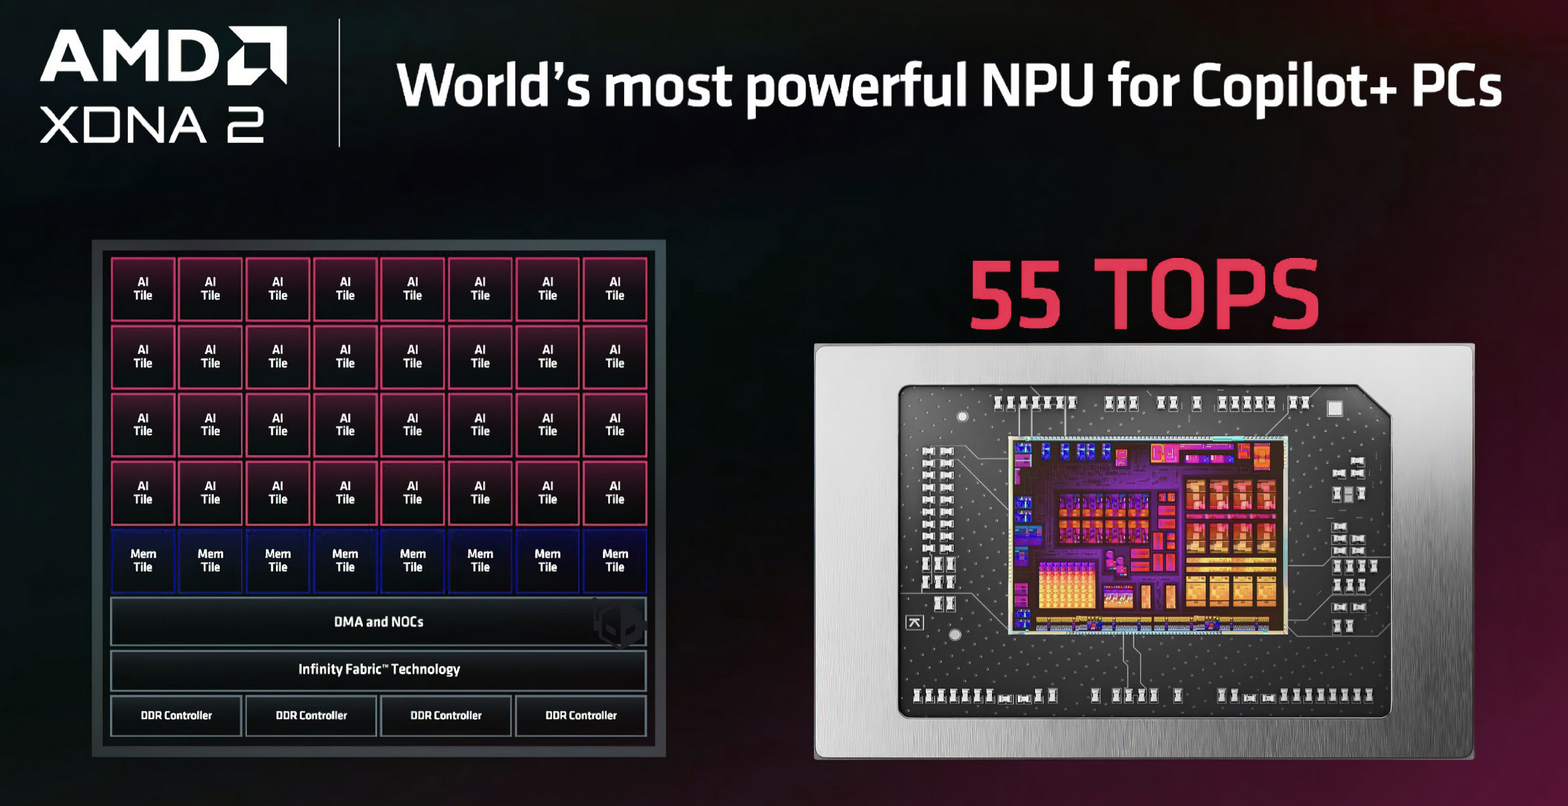
\includegraphics[width=\textwidth]{amd-npu}
                \caption{AMD Ryzen AI}
            \end{subfigure}
        \end{center}
    \end{figure}
\end{frame}

\begin{frame}{Coming back to Von Neumann}
    Specialized hardware is what makes most modern AI systems practical, but it has not replaced the Von Neumann architecture.

\vspace{0.5em}
    Look at any modern computer, even a real AI computer in a data center.
    \begin{itemize}
        \item A CPU sits at the center
        \item GPUs, TPUs, or NPUs attach as accelerators through the bus
        \item All share access to memory, coordinated by the OS on the CPU
    \end{itemize}

    \vspace{0.5em}
    The CPU is still the executive chef.
    The accelerators are highly skilled sous chefs hired for one specialty.
\end{frame}


\section{Exercise}

\begin{frame}{Run a model on different hardware}
    The point of the exercise is to feel the difference between CPU and GPU on the same model.
    Use Google Colab or AI-LAB, and reuse the image classification setup from Module A.4.

    \begin{block}{Outline}
        \begin{enumerate}
            \item Move the model and a batch onto whichever device the runtime exposes via \texttt{.to(device)}, where device is \texttt{"cuda"} or \texttt{"cpu"}
            \item Switch the runtime between CPU and GPU. Restart and rerun after each switch
            \item Time how long one image takes on each device. Average over a few runs, since the first run has warm-up overhead
        \end{enumerate}
    \end{block}
\end{frame}

\begin{frame}{Extensions}
    \begin{enumerate}
        \item Print the parameter count and estimate the model's memory footprint at 4 bytes per parameter
        \item Switch to a heavier model like ResNet-152 or a HuggingFace ViT and repeat the timing. The CPU-GPU gap should grow
        \item Run a small batch of images at once. GPU performance scales with batch size much better than CPU performance does
    \end{enumerate}

    \vspace{0.5em}
    By the end you should have a hands-on feel for why specialized hardware matters, and a number you can point to next time someone tries to sell you an AI computer.
\end{frame}


\appendix

\begin{frame}[plain,noframenumbering]
\begin{center}
{\large Thank you!}
\vspace{1cm}
\\[0.5em]
{\small \faEnvelope\ \href{mailto:lyan@cs.aau.dk}{lyan@cs.aau.dk} \\
\faGlobe\ \href{https://www.yanlincs.com}{www.yanlincs.com}}
\end{center}
\end{frame}

\end{document}
